\section{Join Reordering without statistics}\label{sec:jo}
In the previous section we looked into the current state of affair for Join Reordering and why would it not work for Big Data systems. We will like to propose a novel approach in this section to reorder multi-way Joins just based on the table sizes without any elaborate Table or Column Statistics as required by existing approaches.
We have implemented this approach in Apache Spark and will show how our approach gives upto 85\% improvement on TPC-DS benchmark.

\subsection{Heuristics}

Let us look at the assumptions and heuristics used for the approach.

\subsubsection{Assumptions}\label{subsubsec:assumption}:

\begin{itemize}
\item In Fact-Dimension Join, the Dimension table’s primary key will be joined with the Fact table’s foreign key.
\item Cardinality of Fact Table joined with Filtered Dimension table will be less than that of the Fact table.
\item So based on the last assumption, it follows that if Fact Join with Filtered Dimension happens earlier in multi-way join, it can benefit later joins.
\end{itemize}

To illustrate assumption above, let's look at this query:
\texttt{select * from fact\_table f join dim1 d1 on f.k1 = d1.pk join dim2 d2 on f.k2 = d2.pk where d2.date = ‘06-10-2019’}. If there is a filter on \texttt{dim2} which is smaller than \texttt{dim1} assumption is, it’s join with \texttt{fact\_table} would be smaller than \texttt{fact\_table}. Hence, joining \texttt{fact\_table} with \texttt{dim2} and then with \texttt{dim1} will be beneficial.

As the approach is based upon find Fact-Dimension Join and finding Dominant Fact table in multi-way join, we will look at the heuristics used to find the Dominant Fact table in the following subsection.

\subsubsection{Heuristics for detecting Dominant Fact table}
In the lack of relations information and statistics, we have to use only table sizes and query structure to determine Fact table in a Join. We are using the following heuristics to determine them:

\begin{itemize}
\item At least half of joins in the query should be inner join involving only one table. That would be the Fact table. Other tables being joined with Fact table would be considered Dimension table. Both of them need to satisfy the following constraints.
\item The ratio of the size of the largest Dimensions table to Fact table size should be lesser than a certain threshold. We have used 0.3 as the threshold but it is configurable.
\item None of the Dimensions tables should be partitioned.
\end{itemize}

\subsubsection{Constraints for the Join Reorder algorithm}
We will define all the constraints or boundary conditions for the applicability of the algorithm here:

\begin{itemize}
\item \textbf{Fact Table Constraint}: Only if Dominant Fact table can be determined from multi-way join then we can apply the approach.
\item \textbf{Simple Join Constraint}: Only INNER Joins are considered which can be composed of other Joins too. But apart from the Joins, none of the operator in both the left and right side should be non-deterministic, or have output greater than the input to the operator. For instance, Filter would be allowed operator as it reduces the output over input, but a project adding extra column will not be allowed. It is difficult to reason about operators that add extra to output when dealing with just table sizes.
\item \textbf{Shuffle Constraint}: For systems having shuffle like Spark or Hive, we reorder only if the number of shuffles do not increase due to it. For e.g., consider the following query: \texttt{select * from store\_sales s, item i, web\_sales ws, customer c where s.ss\_item\_sk = i.i\_item\_sk and i.i\_item\_sk = ws.i\_item\_sk and c.c\_customer\_sk = s.ss\_customer\_sk}
\item \textbf{Size Constraint}: Fact table should be at least $X$ times larger than dimension tables. $X$ is configurable. For our implementation Dimension size to Fact size  ratio should be lower than 0.3.
\end{itemize}


Based on above constraint let's look at the core algorithm for finding the optimal Join order. It uses following utility functions based on constraint and heuristics defined above:

\begin{itemize}
\item $hasDominantFact$, $isSimpleJoin$, $obeysShuffleConstraint$: These functions check the constraints defined above. Satisfying these constraints is the pre-requisite to the algorithm.
\item $extractFactDimensions$ will extract Fact table and Dimension Tables for it. This is based on the heuristics defined above.
\item $getFilteredDimensions$ will get us the tables with filter condition upon them based on the list of tables provided to it.
\end{itemize}

\subsection{Algorithm}

\begin{algorithm}
\begin{algorithmic}[1]
\STATE  $\Omega$ $\gets$ $R_1$ $\Join$ $R_2$
\IF{$hasDominantFact$($\Omega$) and $isSimpleJoin$($\Omega$) and $obeysShuffleConstraint$($\Omega$)}
    \STATE $type$ $\gets$ $treeType$($\Omega$) \COMMENT{$type$ will be either $left-deep$ or $right-deep$}
    \STATE ($\sigma$, $\delta$[$1$, $\ldots$, $n$]) $\gets$ $extractFactDimensions$($\Omega$)
    \STATE $\theta$[1, $\ldots$, k] $\gets$ $getFilteredDimensions$($\delta$[$1$, $\ldots$, $n$])
    \STATE $\pi$[1, $\ldots$, l] $\gets$ ($\delta$[$1$, $\ldots$, $n$] - $\theta$[1, $\ldots$, k]
    \STATE $\theta$[k+1] $\gets$ $dummyTable1$
    \STATE $dummyDim1$.$size$ $\gets$ $\infty$
    \STATE $\pi$[l+1] $\gets$ $dummyTable2$
    \STATE $dummyTable2$.$size$ $\gets$ $-\infty$
    \STATE $i$ $\gets$ 0
    \STATE $j$ $\gets$ 0
    \FOR{$r$ $\gets$ $1$ to $n$}
        \IF{$\theta$[$i$].size $\geq$ $\pi$[$j$].size}
            \STATE $i$ $\gets$ $i$ $+$ $1$
            \STATE $result$[$r$] $\gets$ $\theta$[$i$]
        \ELSE
            \STATE $j$ $\gets$ $j$ $+$ $1$
            \STATE $result$[$r$] $\gets$ $\pi$[$j$]
        \ENDIF
    \ENDFOR
    \STATE $\Omega$ $\gets$ $buildJoinTree$($type$, $\sigma$, $result$[$1$, $\ldots$, $n$])
\ENDIF
\RETURN $\Omega$
\end{algorithmic}
\label{algorithm}
\caption{Algorithm to Reorder Joins}
\end{algorithm}


In the algorithm presented above, $\Omega$ is assigned to the input Join that needs to be reordered. Following are the summary of steps to reorder them:
\begin{itemize}
\item Check if all constraints are satisfied for a join: \textbf{Fact Table Constraint}, \textbf{Simple Join Constraint}, \textbf{Shuffle Constraint}, \textbf{Size Constraint}.
\item Once we find Fact table, Join tree associated with it can either be \textit{left-deep} or \textit{right-deep}. Obtain the information as we would like to construct reordered join the same way.
\item Extract the Fact table: $\sigma$ and Dimension tables: $ (\delta_1, \delta_2, \ldots, \delta_n)$. For dimension table, $\delta_i$ represents  $i^{th}$ dimension table being joined with the fact table $\sigma$ from the bottom of the Join Tree as shown in Figure \ref{left-deep}. As the tree here would be either \textit{left-deep} or \textit{right-deep} every dimension will have unique $i$ assigned to them.
\item Split dimensions into two lists: one with selective predicates. $\theta$ and another without it, $\pi$.
\item Sort the list with selective predicates i.e., $\theta$ based on sizes of the dimension tables. Sort the other list i.e., $\pi$ using user-provided order.
\item Merge both the list of dimensions by giving user order the preference for tables without a selective predicate, whereas for tables with selective predicates giving preference to smaller tables. When comparing the top of both the lists, if size of the top table in the selective predicate list is smaller than top of the other list, choose it otherwise vice-versa. This is in congruence with the Assumption made earlier in subsection \ref{subsubsec:assumption}.
\end{itemize}

This is a greedy approach where were are trying to do smaller joins with filtered Dimension table earlier than other Joins to improve Join performance. But in doing so, we take utmost care to not introduce any regression at the same time.

\begin{figure}[ht]
\centerline{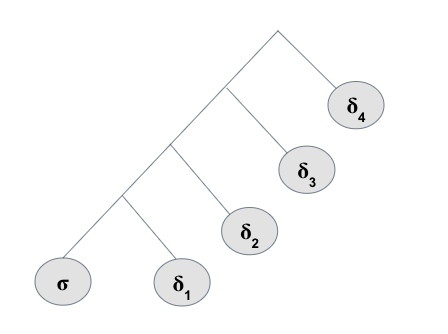
\includegraphics[width=5cm]{fig/left-deep.png}}
\caption{Left-Deep Tree with Fact table $\sigma$ and dimension tables $\delta_i$}
\label{left-deep}
\end{figure}

